Drift detection of corrupted samples for the problem of the thesis has been performed using \textit{alibi-detect} open source python library, that focuses specifically on outlier, adversarial and drift detection algorithms (\cite{alibi-detect}). This library implements statistical hypothesis testing algorithms for detecting drifts in data. 

It works the following way, before observing some data, one can specify null-hypothesis $H_0$ and alternative hypothesis $H_1$ about generating process behind the data (its distribution for example) and also specify the test statistics $S(X)$ that are expected to be small under hypothesis $H_0$ and large under hypothesis $H_1$. Then during the observation of the new data test statistic value $S(X)$ is computed along with a probability $p = P(S(X)|H_0)$ which is called p-value. P-value is a probability that such an extreme value of test statistic could have been observed under the null-hypothesis. If this probability is below the established threshold $t$, then one can assume that data is drifted. If p-value is low, null-hypothesis will be refused. 

We have trained a drift detection algorithm on UNet embeddings of not corrupted train data. For this experiment $5000$ embeddings were used of CHZN and PHX phenotypes from the nucleus dataset. After the drift detection algorithm was trained, we tested it on the test dataset, that was not seen by a model beforehand. Test dataset consists of 119 images, where from each image $5$ random crops were chosen. Since images have a high resolution, one can assume that one image itself represents a new input distribution, where crops taken from this image are its samples. Therefore we can detect whether one specific image has drifted or not feeding the crops from it into a drift detection algorithm. First, the algorithm was tested on not drifted data by using a test set of nucleus dataset. Out of $119$ images $10$ were recognized as drifted ones. This means that the algorithm's false positive is approximately $\frac{10}{119} \approx 0.08$. Figure \ref{fig:fn-rate} presents the results of drift detection for all artificial corruptions, more specifically the algorithm's false negative rate.
\begin{figure}[H]
	\begin{center}
		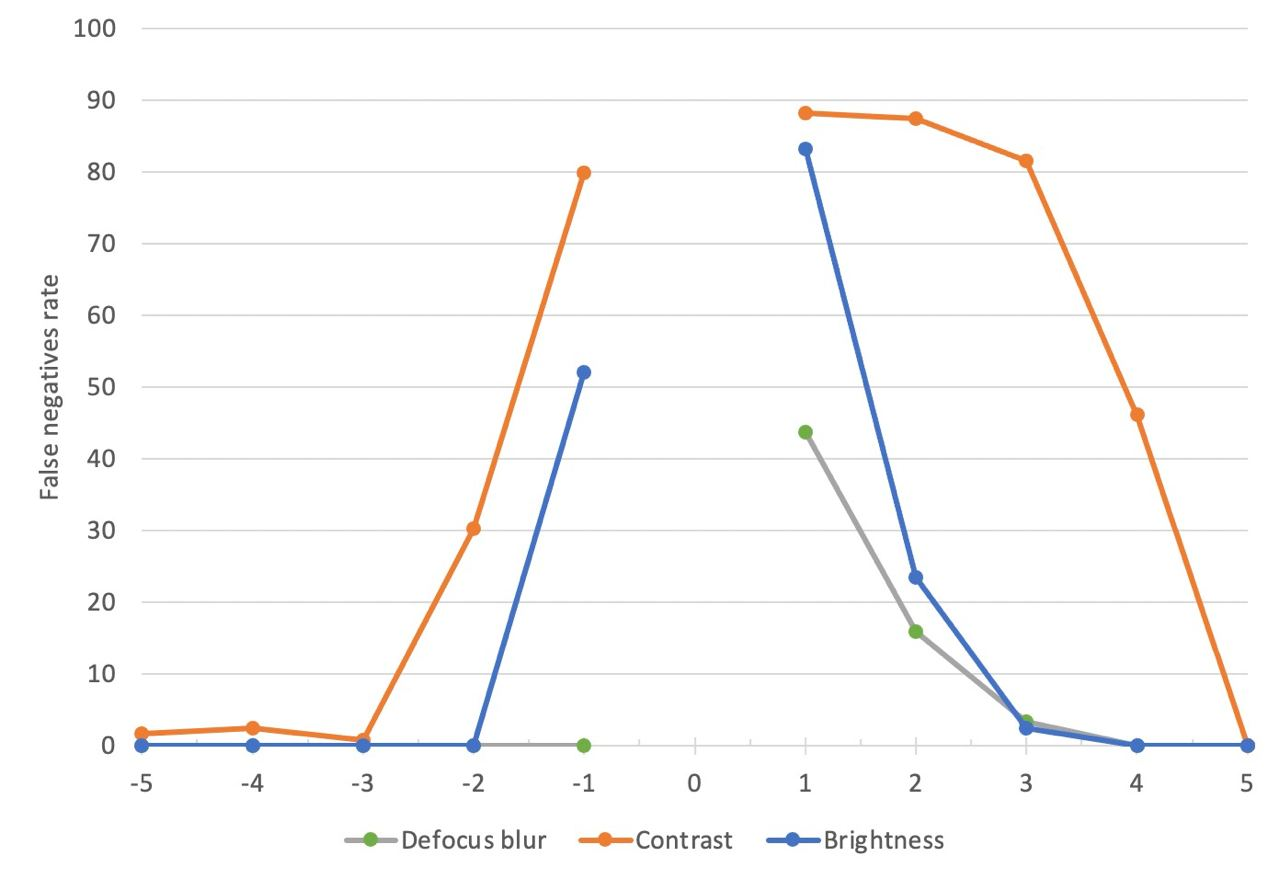
\includegraphics[width=0.5\linewidth]{bilder/drift-detection/fn-rate.jpg}
		\caption{False negatives rate for drift detection on artificial corruptions}\label{fig:fn-rate}
	\end{center}
\end{figure}
One can see that the lower the severity of a corruption is, the higher the false negative rate becomes. When the corruption severity level is low the predictions remain to have a high quality (see Figure \ref{fig:artificial-corruptions}), therefore an end user can still rely on the UNet. However, the stronger the corruption is, the stronger fluorescence prediction degenerates and as a result a drift detector alerts a user to the presence of drift. Drift detector is more sensitive towards contrast changes rather then towards brightness changes. It is the most sensitive towards defocus blur corruption, which alings well with the visual examinations, where it is clear that defocus blur has the most influence on fluorescence predictions.